\subsubsection*{Le matin :}
La matinée à été passée a comenter le code afin de simplifier son utilisation.
Ee nouvelles loss functions ont été codées.


\subsubsection*{L'après midi :}
Une réunion a eut lieu avec Johanne :
les résultats sont bons mais pour pouvoir dire plus de choses, il serait bien de tracer un graphique ecart type de l'erreur de l'apprentissage en fonction de : la taille de la base de donnée, le trie des données et la normalisation dans la loss function.\\
De nouvelles fonctions ont donc été codées dans ce but.

Théoriquement, l'écart type devrais diminuer quand la taille de la base de donnée augmente.

\begin{figure}[H]
    \center
    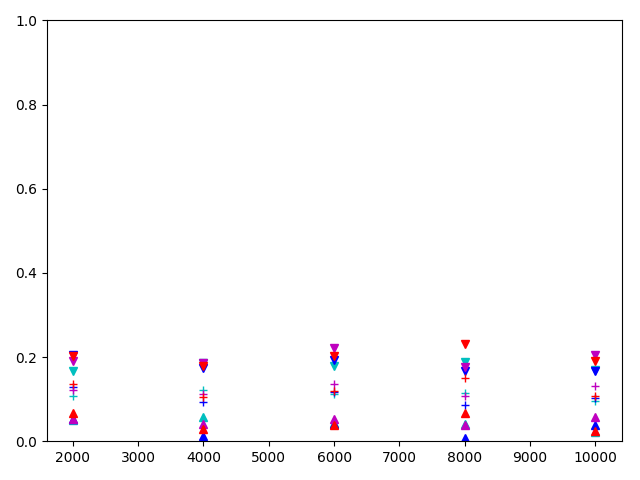
\includegraphics[height=\grand]{sources/data/etfdata/graph1}
	\caption{Ecart type de l'apprentissage en fonction de la taille de la base de données}
	\label{etfdata1}
\end{figure}
On peut bien voir qu'avec les données ci dessus, l'echantillon est trop petit pour voir une variation de l'ecart type: les diferences ne sont pas significatives.
On refait l'experience avec les tailles suivantes en entrée : $10$, $50$, $100$, $500$, $1000$, $5000$, $10000$.
Le calcul prend du temps, j'aurais les resultats demain matin.

